\section{Dominant Background: Standard Model $t\tbar$}
\label{sec:Bkg:ttbar}

\indent The dominant background in this analysis is standard model ttbar.  Section \ref{sec:Bkg:ttbar:Pop} describes the two kinematically distinct populations of ttbar that exist after preselection.  One ttbar population is also produced with strong initial state radiation and the other population does not have strong ISR.  \\
\indent Section \ref{sec:Bkg:ttbar:Sel} describes the signal selections used to remove the majority of ttbar background while retaining most of the signal.  These selection targets the larger and kinematically different population of ttbar that does not have strong initial state radiation.  ttbar with strong ISR appears more signal like and 90 percent of all ttbar backgrounds after signal region selection are ttbar events with at least $400$ GeV of true initial state radiation.  These same selections are also very effective at removing sub-dominate SM backgrounds such as W+jets and Z+jets. \\
\indent Section \ref{sec:Bkg:ttbar:CR} describes how we are able to directly measure the amount of ttbar background that is produced with strong initial state radiation in data using an one lepton control region.  We avoid relying on theory predictions on the amount of ISR ttbar is expected to produce.  In this way, the control region allows us to minimize the amount of systematic uncertainties in the signal region. \\
\indent After signal selection ttbar still accounts for $85$ percent of our background. 80 percent of the ttbar has one top decay via a single hadronic tau and the other top decays fully hadronically.  $15$ percent of the ttbar events decay via the single lepton channel where the lepton is an electron or a muon.  The lepton becomes lost because either it has too low pt to be reconstructed, removed because they were to close to another jet or is mis-reconstructed as a jet. The rest of the five percent composed of di-leptonic or lepton and tau ttbar events. Essentially no fully hadronic ttbar survives the zero lepton selection because fully hadronic ttbar do not make any hard neutrinos directly from the top decay.  The $250$ GeV \MET selection removes all fully hadronic ttbar.  \\

\subsection{Two Kinematically Distinct Populations of $t\tbar$}
\label{sec:Bkg:ttbar:Pop}

\indent Most ttbar events has one top that decays leptonically and the other top decaying fully hadronically after zero lepton preselection. The leptonic top also produces a neutrino that satifies the $250$ GeV of \MET requirement.  In most cases, the lepton is a tau that decays hadronically and registers as jet in calorimeter instead of a lepton.  In a smaller fraction of events a muon or electron is produced but the lepton is lost because of a number of reasons.  For example, the lepton can have too low pt to be reconstructed, or can be removed because they were to close to another jet or an electron is mis-reconstructed as a jet.  \\
\indent Regardless of the exact decay channel, a top decaying at rest cannot generate enough momenta for the neutrino to have $250$ GeV of pt.  The top decaying via a tau or lepton, called the leptonic top, must therefore be boosted to have a high probability of satisfying the $250$ GeV \MET cut.  The leptonic top can gain this boost through one of two ways.  Either the leptonic top recoils in a back to back fashion against the hadronic top or both tops recoil against strong ISR.  \\
\indent In both situations the axis of maximum back to back momenta, the thrust axis, contains important information.  In the case where the leptonic is recoiling against the hadronic top, the thrust axis lines up along the two top's back to back recoil.  In the case where both tops are boosted by strong ISR, the thrust axis lines up along the direction of the two tops' recoil against strong ISR. A basic representation of the kinematics of the two populations and the role of the thrust axis in each of them can be seen in figure \ref{fig:ttbar:2pop}. \\
\indent One can clearly see that the two population has very different kinematics once we divide the event in half along the thrust axis.  \\
\begin{figure}[h!]
  \centering
	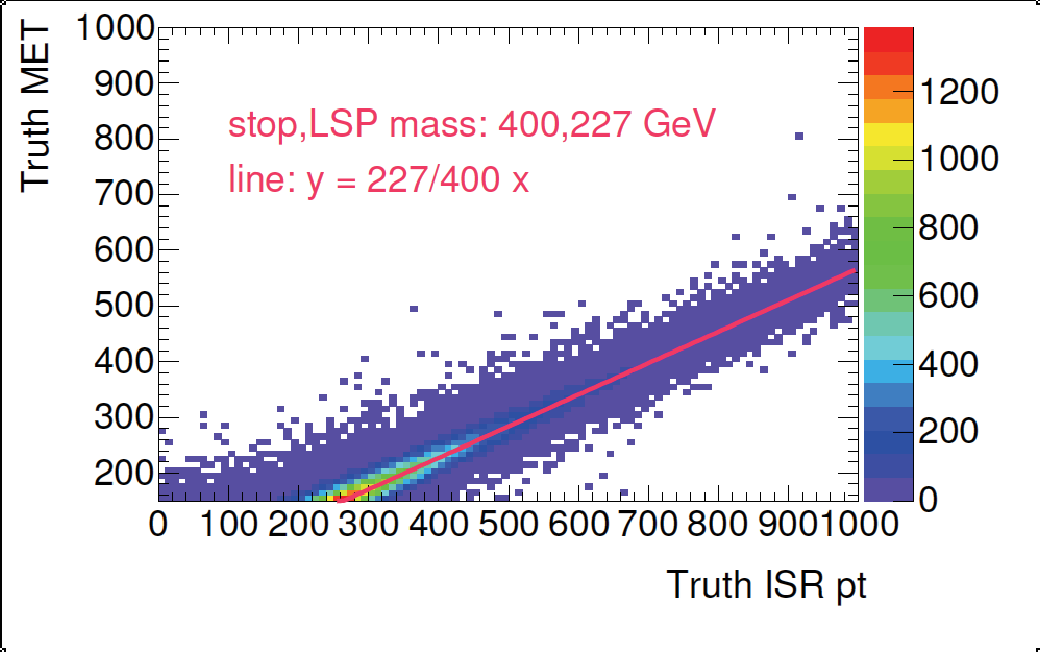
\includegraphics[width=0.65\textwidth]{./figures/MET_ISR.png}
\caption{\label{fig:ttbar:2pop}{Basic depiction of the kinematics of the back to back ttbar population and the ttbar plus strong ISR population that exists after the zero lepton pre-selection. }}
\end{figure}

\subsection{Properties of $t\tbar$ in Signal Region}
\label{sec:Bkg:ttbar:SR}

\indent The ttbar events that survives the signal region selection is almost completely ttbar events also produced with strong initial state radiation.  In the signal region, 90 percent of the ttbar events have at least 400 GeV of ISR pt.  The distribution of true ISR pt for ttbar that survive the signal selections can be seen in figure \ref{fig:ttbar:SR:trueISRpt}.\\

\begin{figure}[h!]
  \centering
	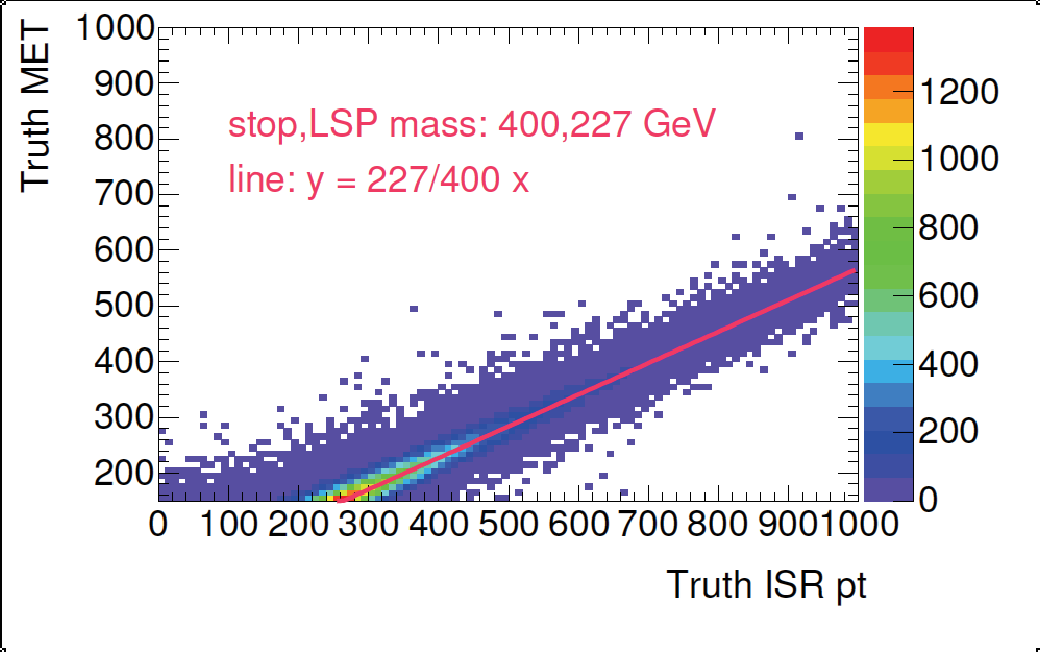
\includegraphics[width=0.65\textwidth]{./figures/MET_ISR.png}
\caption{\label{fig:ttbar:SR:trueISRpt}{Distribution of true ISR pt for ttbar that survive the signal selections}}
\end{figure}

\indent In terms of branching fractions, the majority of ttbar branching fractions are to hadronic taus.  80 percent of the ttbar has one top decay via a single hadronic tau and the other top decays fully hadronically.  $15$ percent of the ttbar events decay via the single lepton channel where the lepton is an electron or a muon.  The lepton becomes lost because either it has too low pt to be reconstructed, removed because they were to close to another jet or is mis-reconstructed as a jet. The rest of the five percent composed of di-leptonic or lepton and tau ttbar events. Essentially no fully hadronic ttbar survives the zero lepton selection because fully hadronic ttbar do not make any hard neutrinos directly from the top decay.  \\
\indent With such a large fraction of background coming from taus one might suspect setting up some sort of tau rejection.  However we found that a rejection based on loose tau IDs did not improve sensitivity.  The loss of signal was too large to justify the improvement in signal to background ratio.  The high jet multiplicity in signal gives a high probability of false positives.
\indent Accepting mainly ttbar decay to hadronic taus gives a large boost signal to background due to branching fractions alone.  The two tops in signal events decay mainly through the fully hadronic channel.  Fully hadronic decays accounts for 44 percent of all ttbar decays.  On the other hand, the ttbar background mainly decay via hadronic taus which only accounts for about 10 of all ttbar decays.  We therefore gain a factor of 5 in signal to background ratio just by working in the zero lepton channel. This not only gains us a great boost in sensitivity in our signal region.  It also allows us to design a ttbar control region with very similar selections to the signal region but just in the single lepton channel.  We can avoid high signal contamination in our control region because both signal and background are mainly coming from single lepton decays in the 1 lepton channel.  As such, we no longer gain this factor of 5 in S/B based on branching fraction in the control region.  The details of the ttbar control region is described in section \ref{sec:Bkg:ttbar:CR} \\  

\subsection{Predicting the amount of $\ttbar$ in Signal Region using a One Lepton Control Region}
\label{sec:Bkg:ttbar:CR}

\indent The ttbar that populate the signal region is mainly ttbar produced with strong initial state radiation as shown in section \ref{sec:Bkg:ttbar:SR} and \ref{sec:Bkg:ttbar:Sel}.  A direct consequence of this is that our predictions for the amount of background in our signal region is directly related to the amount of ISR/FSR in our ttbar MC.  The next-to-leading order (NLO) MC simulations of ttbar gives upwards of 30 to 35 percent uncertainty in the amount of predicted ttbar background in the signal region (SR).  This theoretical uncertainty would be our single largest uncertainty if we had to rely on theoretical calculations alone.  Instead we directly measure the amount of ttbar that is produced with strong ISR in-situ directly from ATLAS data using an one lepton ttbar control region (ttbar CR).  Using the ttbar CR we are able to reduce the ISR/FSR systematic uncertainty in the SR down to a manageable 10 percent in all signal regions.\\
\indent The selections used to define the ttbar CR is defined in table \ref{tab:ttbar1LepCRISR_def}.  This control region is designed using the same sensitive variables as the SR definition to mimic the signal regions as close as possible while maintaining a high purity of the dominant background semi-leptonic \ttbar.  The CR is defined in the 1 lepton channel where the lepton is a signal muon or signal electron.  The lepton is included as a "jet" in the Jigsaw ISR algorithm and will be counted as a sparticle jet or an ISR jet depending on which hemisphere it falls.  In this case the lepton is supposed to mimic the hadronic tau jet that exists in 80 percent of all ttbar events.\\

\begin{table}[htpb]
  \caption{One-lepton \ttbar+ISR control region (ttbar CR) definitions. The same \met\ triggers as mentions in Table~\ref{tab:SRcommon} are used. }
  \begin{center}
    \def\arraystretch{1.4}%
    \begin{tabular}{c|c} \hline\hline
      {\bf Variable}     & 1L 1b \ttbar CR \\ \hline \hline
      1 Lepton Pre-Selection & true \\ \hline
      Number of leptons  & 1                   \\
      Number of $b$-jets & $\ge1$              \\
      \mtlepmet          & $<80\gev$           \\ 
      \mindrblep         & $<2.0$              \\ 
      \NjV               & $\ge5$              \\
      \NbV               & $\ge1$              \\
      \pTSFour           & $>40\gev$           \\
      \PTISR             & $\ge 400$           \\ \hline \hline
    \end{tabular}
  \end{center}
  \label{tab:ttbar1LepCRISR_def}
\end{table}%

\indent All variables used are defined in section \ref{Jigsaw:Variables}. A cut of $\mtlepmet < 80\gev$ is added to remove signal contamination and a $\mindrblep<2.0$ cut is added to increase ttbar purity and ensure orthogonality to the W+jets control region. \\
\indent The $\dphiISRI>3.0$ is removed to increase CR statistics. \dphiISRI specifies the direction of neutrino relative to the direction of the ISR.  A requirement on $\dphiISRI>3.0$ essentially selects only specific decay axis that the \ttbar\ decay can take place.  Therefore removing this cut opens up more phase space that the tops can decay in the CR but does not change qualitative property that the \ttbar\ events in the CR must have strong initial state radiation. \\
\indent The $\pTjV>50\gev$ cut is relaxed to $\pTjV>40\gev$ in order to increase statistics in the CR.  The $\pTjV$ cut specifies the \pt\ of the 4th jet in the sparticle system.  Loosening this cut increases statistic by allowing the 4th jet in the \ttbar\ decay to have softer \pt\ but does not change the hardness of $>400\gev$ ISR system.  The $\pTjV$ cut can be correlated with ISR/FSR because there is a chance that the 4th most energetic jet in the sparticle system is from radiation and not a top decay.  However for this analysis it is more important to accurately gauge the amount of hard ISR of order hundred or more GeV that the ttbar recoils against then amount of softer radiation on the \ttbar\ side. We found that a looser $\pTjV$ cut of 40 GeV does not cause a difference in the true ISR pt distribution of the ttbar in the CR and SR. \\
\indent Distribution of important variables after normalization to \intlumi\ \ifb\ of data are shown for ttbar CR in figure \ref{fig:CRTopC}.  There seem to be no significant slope in signal over background between $\pTjV$ distribution.  This allows for the 40 to 50 GeV extrapolation across this variable between CR and SR.  There is a noticeable trend in $\pTISR$.  This is not surprising given that a priori we have an 30-35 percent uncertainty in ISR/FSR systematic.  The ttbar MC alone is a poor predictor of the amount of ISR which is why we do not extrapolate at all across the $\pTISR$ variable.  The disagreement in data and MC in $\pTISR$ further demonstrate the need for a control region that directly measures the amount of ttbar with strong ISR pt directly from data. \\

\begin{figure}[htbp]
  \begin{center}
    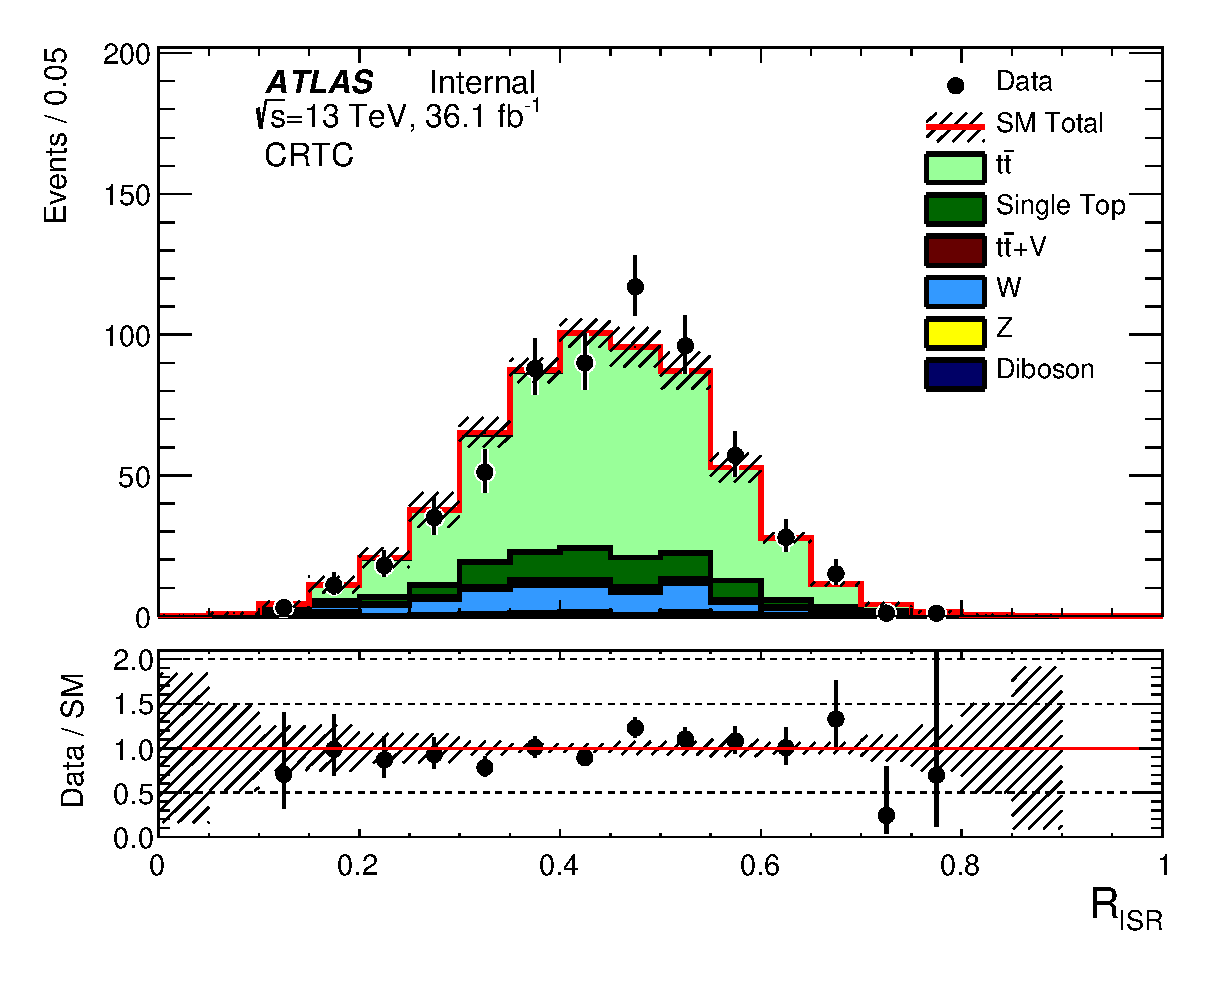
\includegraphics[width=0.45\textwidth]{figures/ttbar/postfit/CA_RISR_CRTopC}
    \includegraphics[width=0.45\textwidth]{figures/ttbar/postfit/CA_pTISR_CRTopC}
    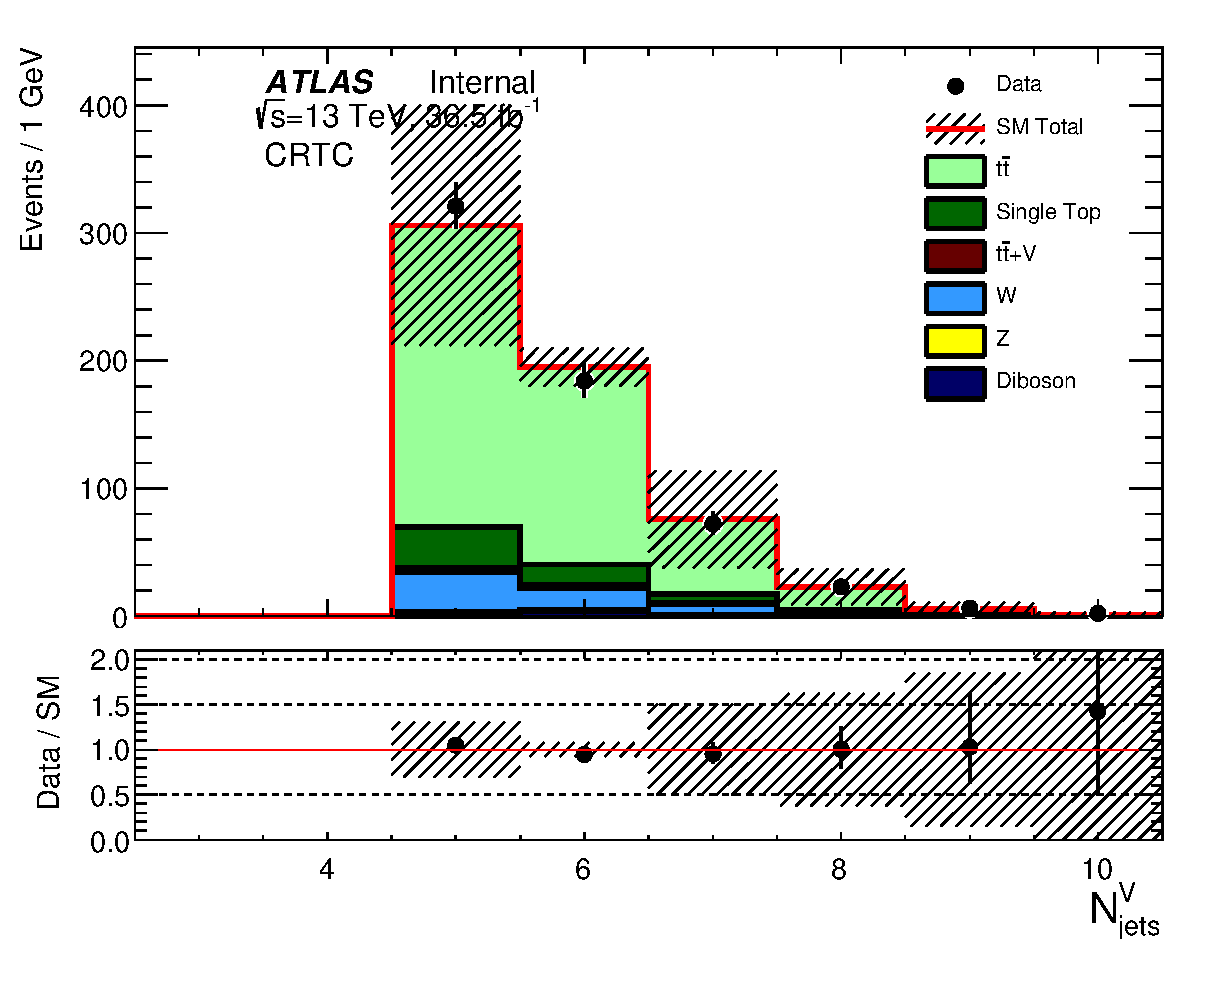
\includegraphics[width=0.45\textwidth]{figures/ttbar/postfit/CA_NjV_CRTopC}
    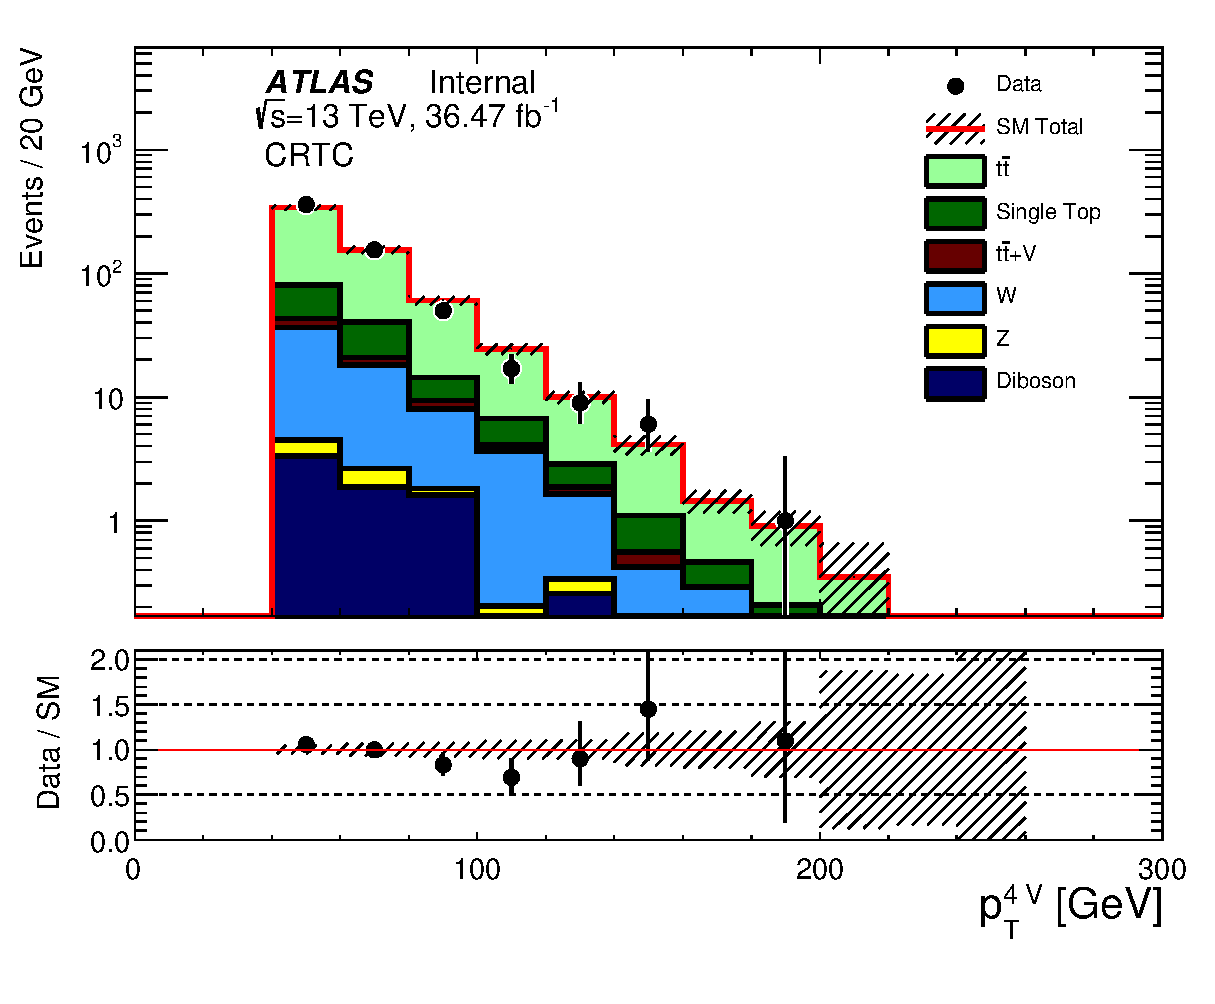
\includegraphics[width=0.45\textwidth]{figures/ttbar/postfit/CA_pTjV4_CRTopC_log}
    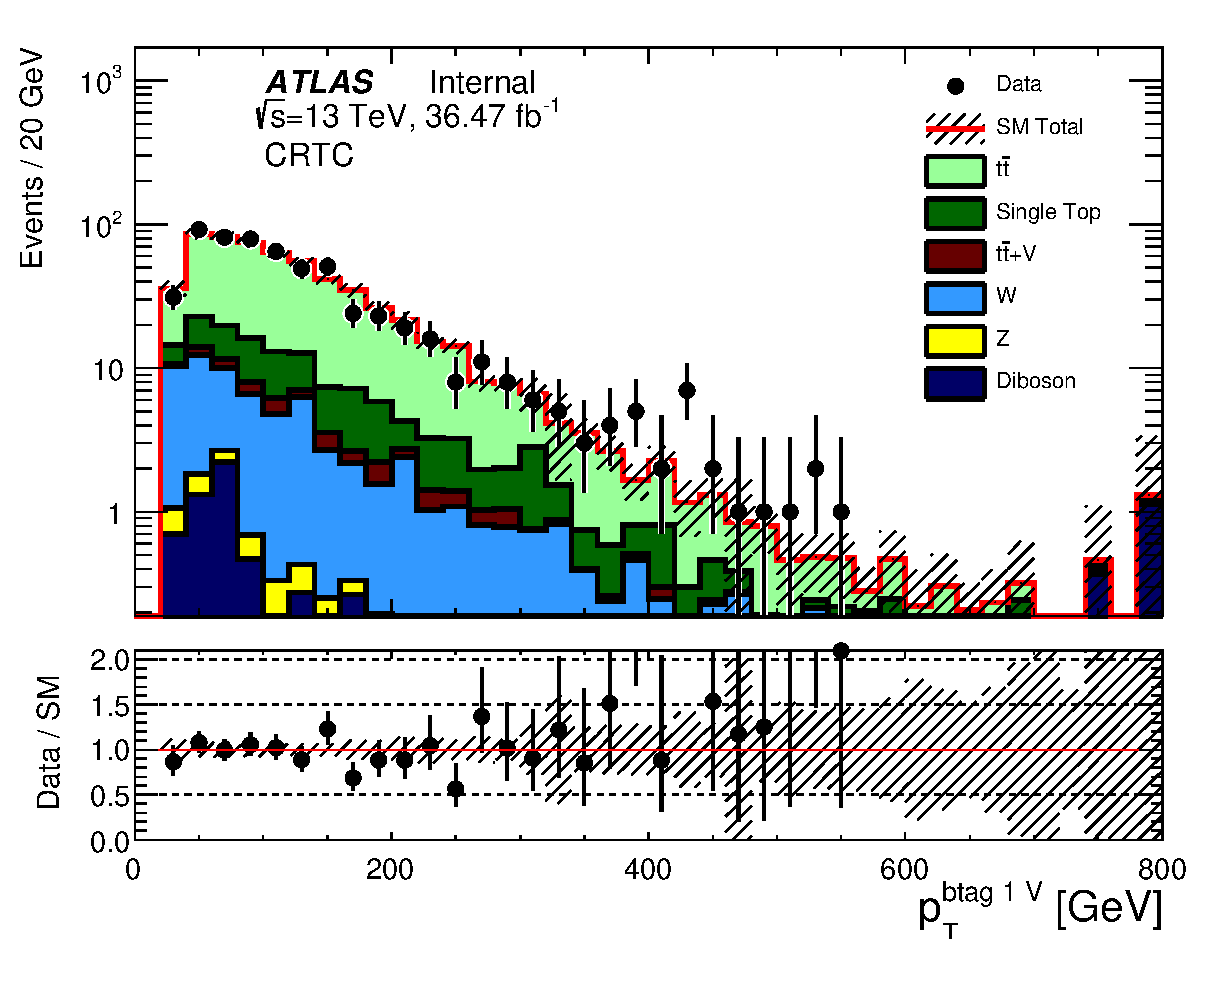
\includegraphics[width=0.45\textwidth]{figures/ttbar/postfit/CA_pTbV1_CRTopC_log}
        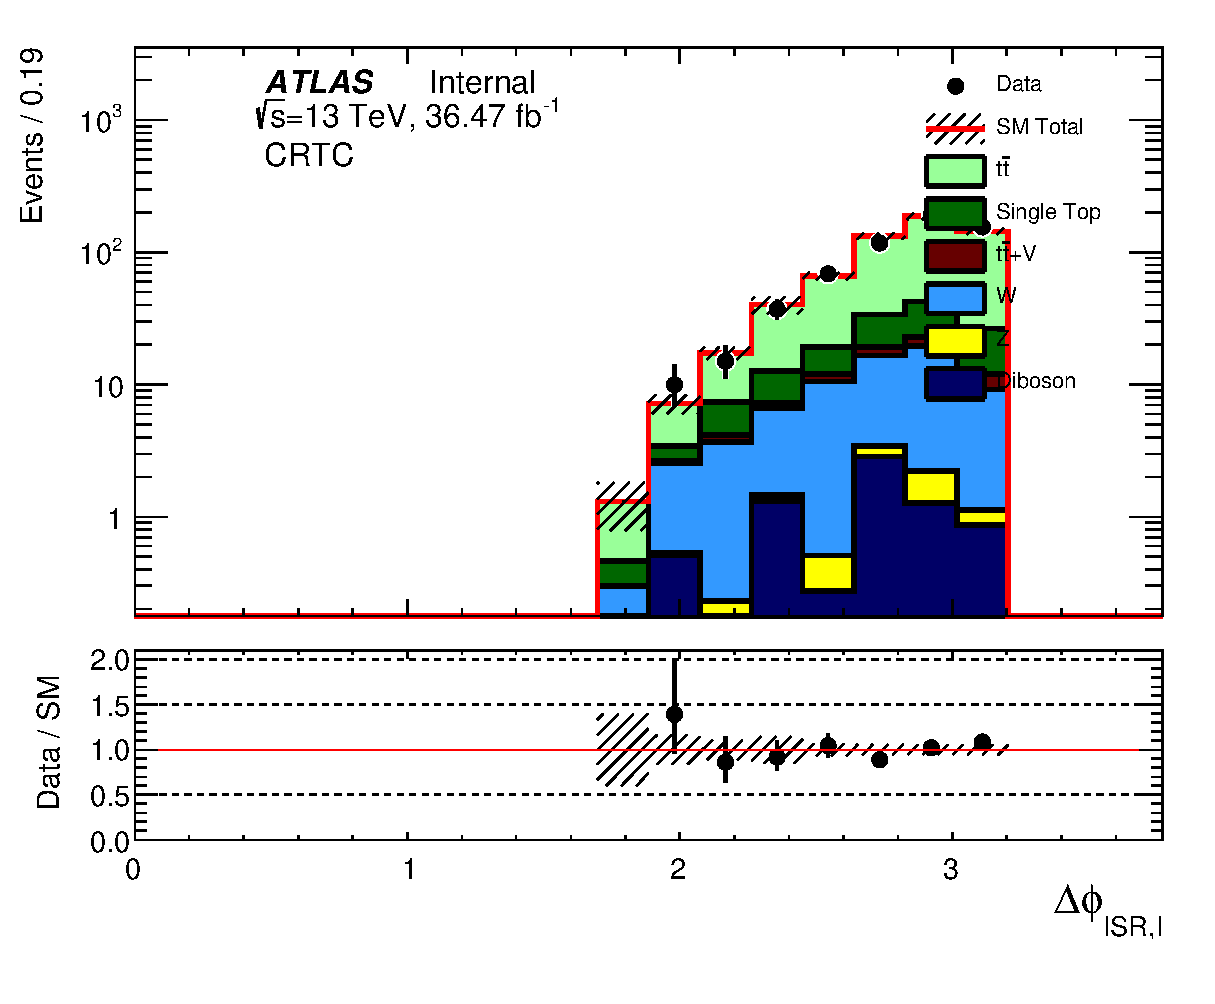
\includegraphics[width=0.45\textwidth]{figures/ttbar/postfit/CA_dphiISRI_CRTopC_log}
  \end{center}
  \caption{ttbar CR postfit distributions for \intlumi\ \ifb\ of data. The ratio between data and MC is shown in the bottom panel. The hashed area in both the top and lower panel represent the uncertainty due to MC statistics and detector systematic uncertainties.}
  \label{fig:CRTopC}
\end{figure}

The true ISR pt distribution of the events in the CR and SR is shown in figure \ref{fig:ttbar:CR:trueISRpt}. The remarkable similarity between the ttbar true ISR pt distribution in CR and SR show that the CR captures the same ttbar plus strong ISR population that dominates the SR.  \\

\begin{figure}[h!]
  \centering
	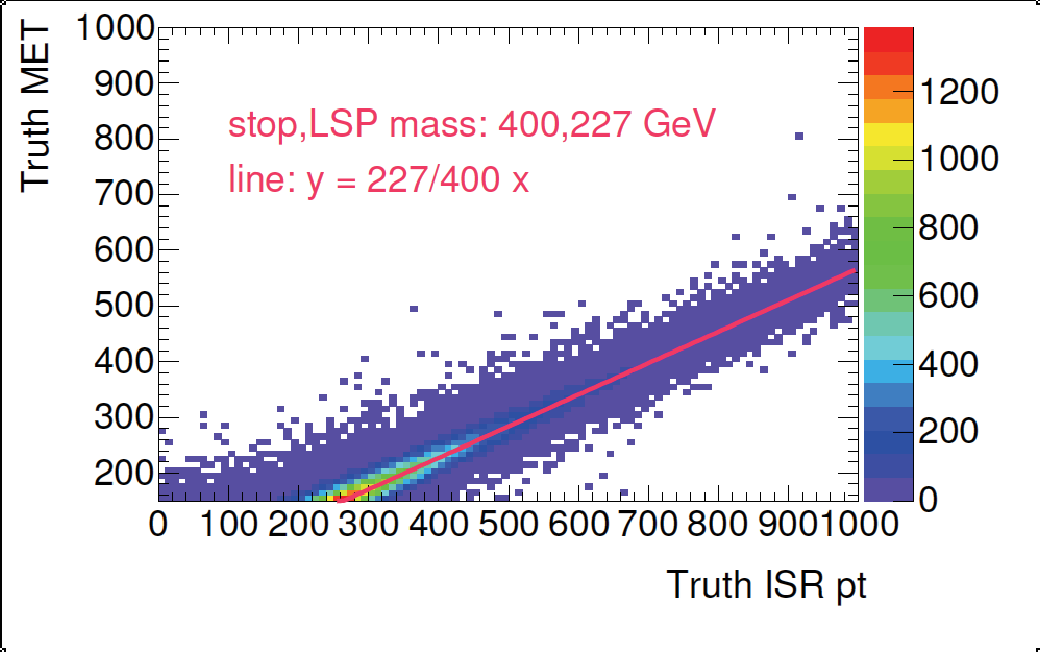
\includegraphics[width=0.65\textwidth]{./figures/MET_ISR.png}
\caption{\label{fig:ttbar:CR:trueISRpt}{Distribution of true ISR pt for ttbar that survive the signal selections and control region selections}}
\end{figure}

\indent We derive the normalization scale factor derived using \intlumi\ \ifb of data for ttbar is 0.73 using the ttbar control region.  Therefore the control region tells us that we need to scaled down the amount of ttbar background predicted by the MC in the SR by a factor of 0.73. \\
\indent This scale factor is quiet different from 1.0 which indicates that the ttbar MC alone does not well model the high ISR pt phase space.  This highlights the importance of a control region that captures the same ttbar+strong ISR population that we see in the 0 lepton SR.  \\
\indent Essentially we place more trust that the MC can predict the relative rates of single lepton and single hadronic tau ttbar then we do in the MC predicting the amount of ISR ttbar produces. This "trust" can be seen in the fact that other systematics such as jet energy scales and lepton ID efficiency are smaller then the ISR/FSR uncertainty.  A more detailed discussion of systematics can be found in section \ref{sec:sys}\\

\subsection{Validating $\ttbar$ Predictions in Signal Region using a Zero Lepton Validation Region}
\label{sec:Bkg:ttbar:VR}

\indent We also want a zero lepton region that is orthogonal but close to the signal in order to validate the prediction made by the one lepton ttbar control region (ttbar CR) .  We call this region the zero lepton ttbar validation region (ttbar VR).  The validation region is designed using the same sensitive variables as the SRC definition to mimic the signal regions as close as possible while maintaining a high purity of the dominant background semi-leptonic \ttbar. \\
\indent The requirement on \MS\ is reduced to 100 GeV (vs. 300 GeV in the SR) and an $\NjV \ge 4$ selection is applied (vs. $\NjV \ge 5$ in the SR) to enhance the yields of semi-leptonic \ttbar\ events . A requirement of $\MV/\MS < 0.6$ is added to both to reduce signal contamination and protect against any remaining QCD multi-jet contribution. Again $\pTjV>50\gev$ cuts are relaxed to $\pTjV>40\gev$ to increase VR statistics. \\
Finally the $\dphiISRI$ cut is inverted to $\dphiISRI<3.0$ to cut out signal and maintain orthogonality to the signal region. We expect ttbar events to have neutrinos that don't go directly opposite the \\ 

\begin{table}
  \caption{Zero-lepton \ttbar+ISR validation region definitions, in addition
    to the SRC requirements listed in Table~\ref{tab:SRcommon}.}
  \begin{center}
    \def\arraystretch{1.4}%
    \begin{tabular}{c||c} \hline\hline
      {\bf Variable} & \\ \hline \hline
      \NjV           & $\ge4$                \\
      \NbV           & $\ge1$                \\
      \pTbV          & $\ge 40$              \\
      \PTISR         & $\ge 400$             \\
      \MS            & $>100\gev$            \\
      $\MV/\MS$      & $<0.6$                \\
      \dphiISRI      & $<3.00$               \\ \hline \hline
    \end{tabular}
  \end{center}
  \label{tab:ttbar0LepVR}
\end{table}%

The distributions of the SRC sensitive variables in the \ttbar+jets zero-lepton validation regions are shown in Fig.~\ref{fig:ttbar0Lep1bVRISR}, with normalizations and systematic uncertainties corresponding to those predicted by the 1L ttbar+ISR CR fitted to \intlumi\ fb$^{-1}$ defined in Table~\ref{tab:ttbar0LepVR}. \\

\begin{figure}[htbp]
  \centering
    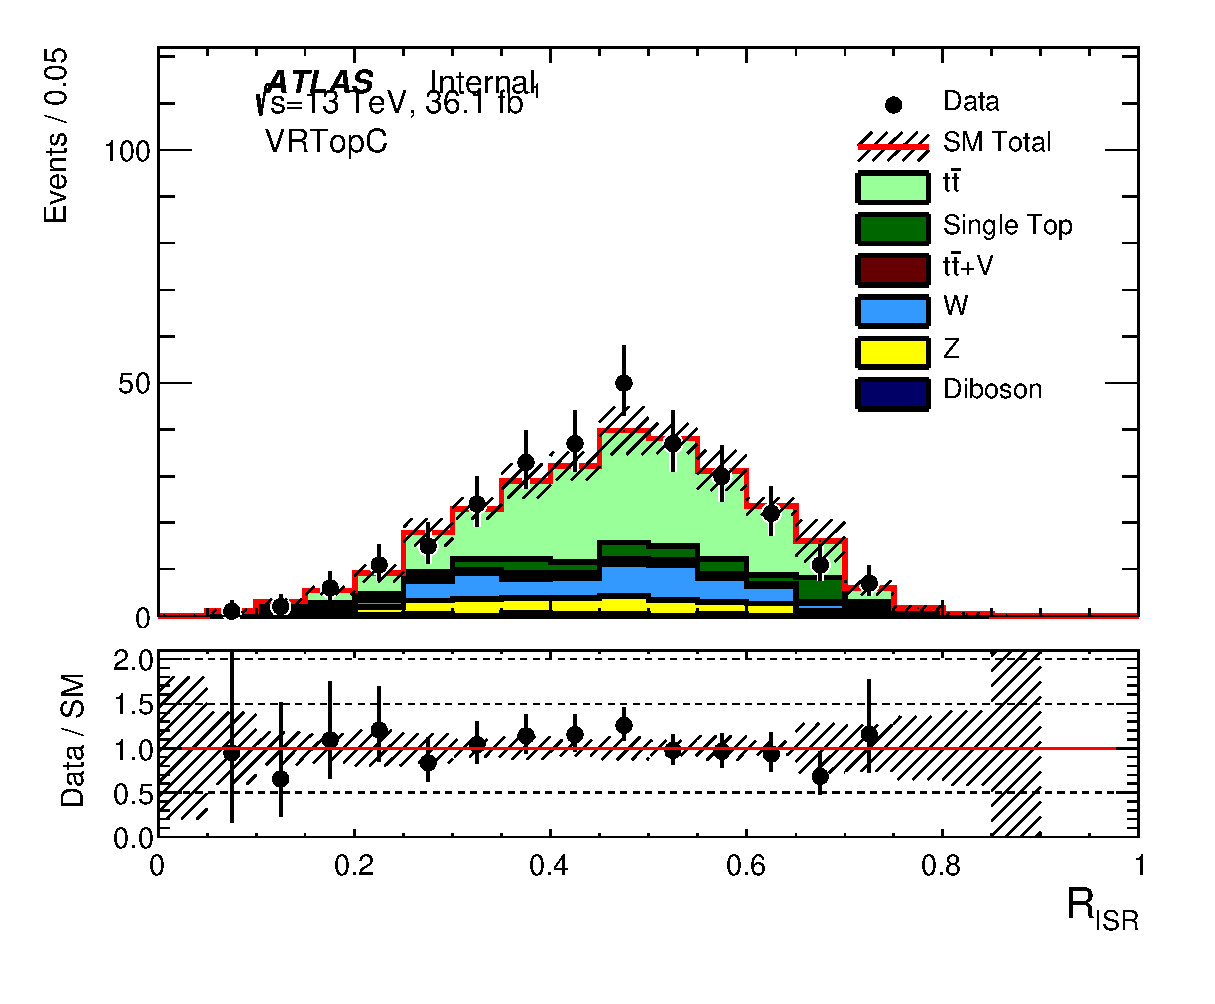
\includegraphics[width=0.45\textwidth]{figures/ttbar/postfit/CA_RISR_VRTopC}
    \includegraphics[width=0.45\textwidth]{figures/ttbar/postfit/CA_pTISR_VRTopC}
    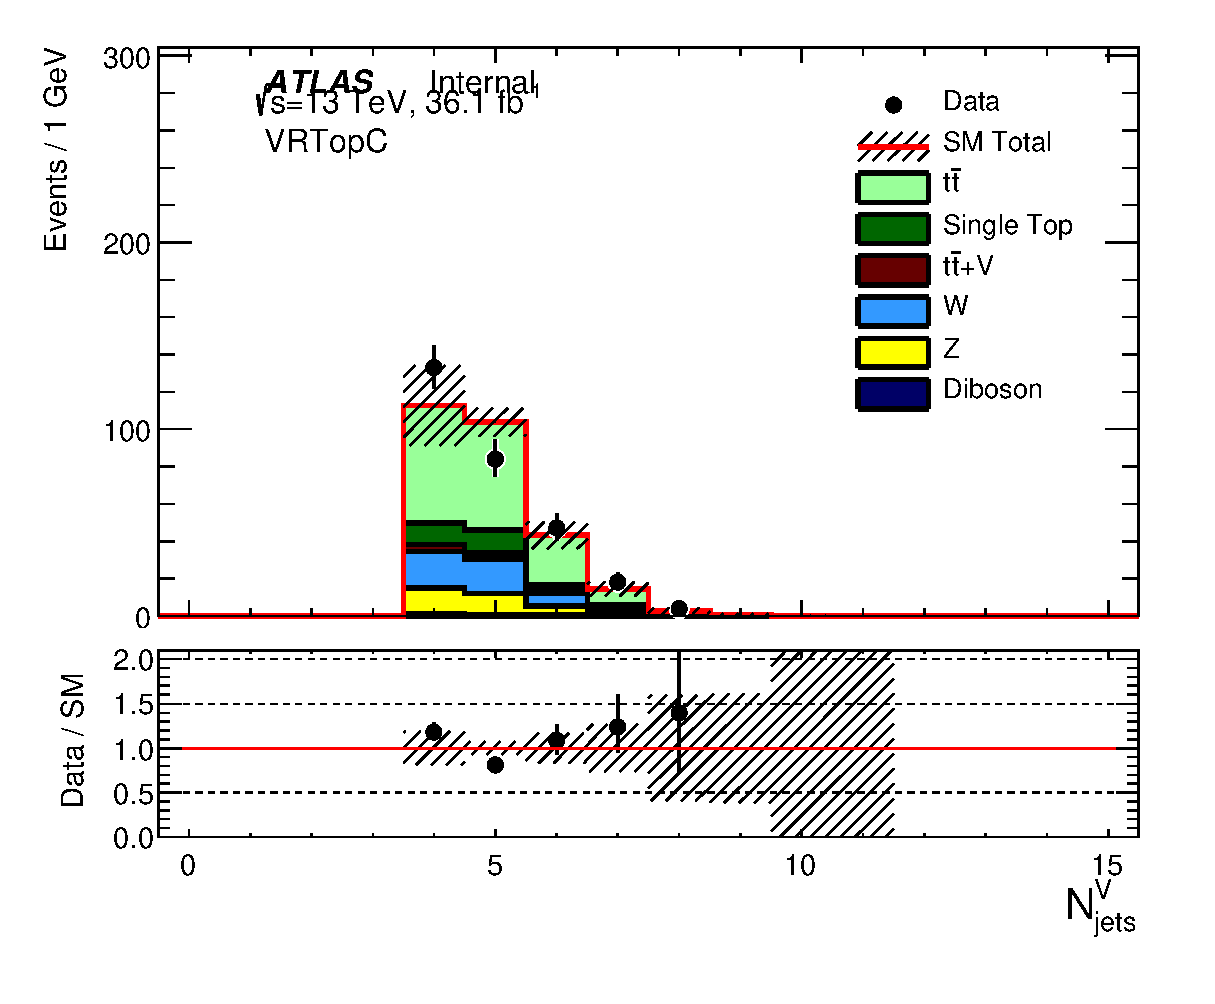
\includegraphics[width=0.45\textwidth]{figures/ttbar/postfit/CA_NjV_VRTopC}
    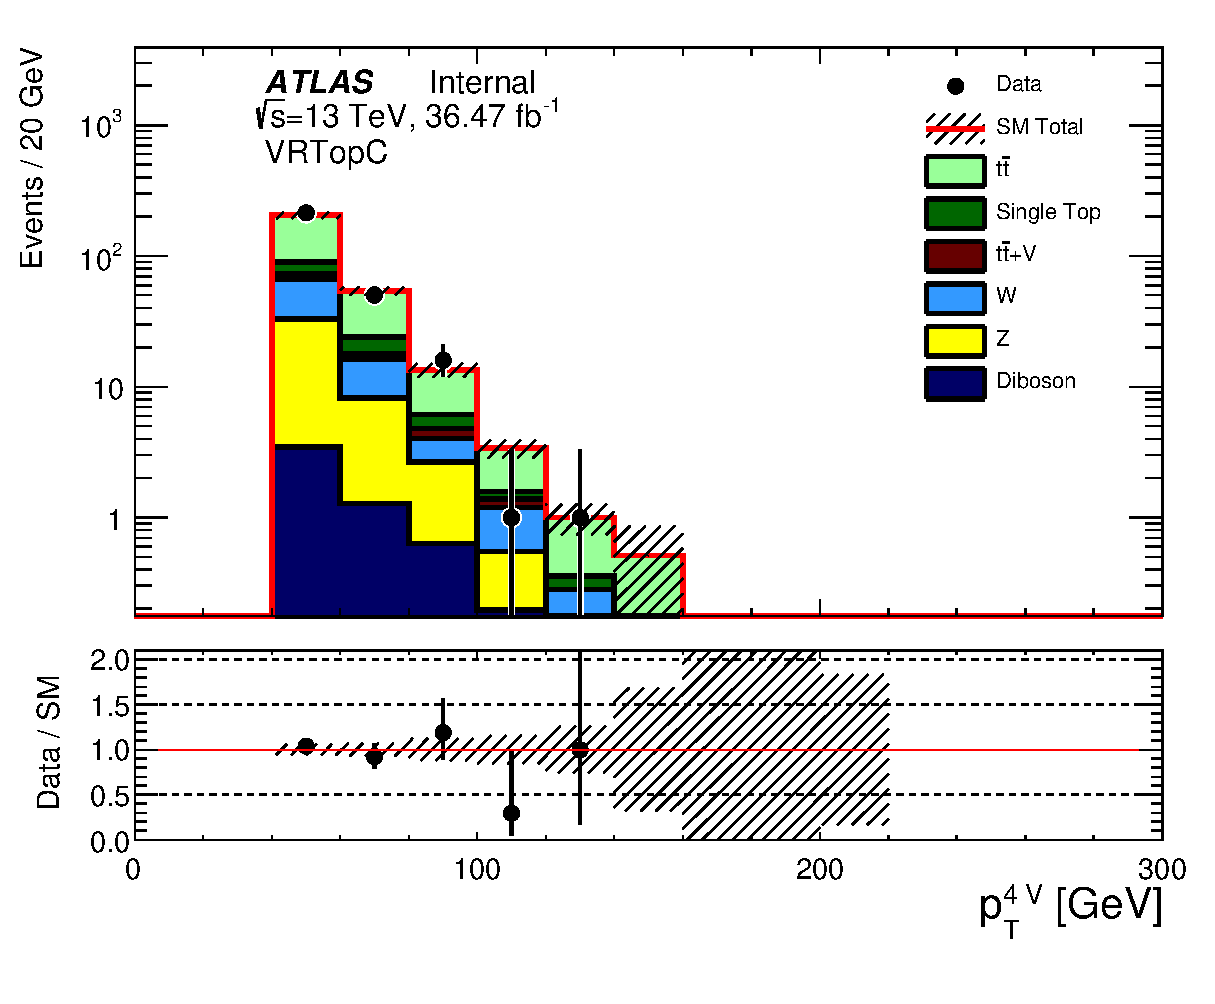
\includegraphics[width=0.45\textwidth]{figures/ttbar/postfit/CA_pTjV4_VRTopC_log}
    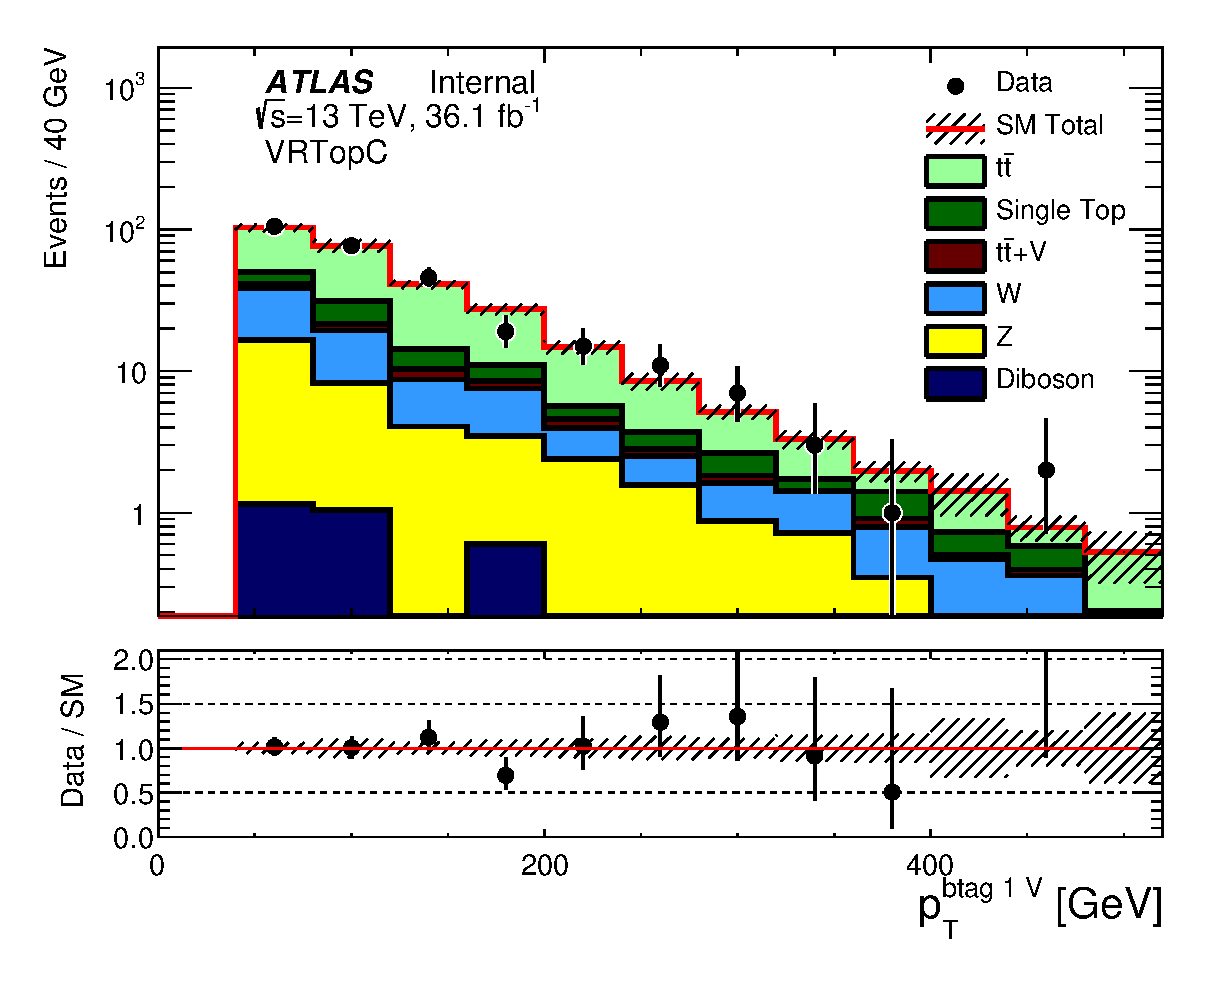
\includegraphics[width=0.45\textwidth]{figures/ttbar/postfit/CA_pTbV1_VRTopC_log}
        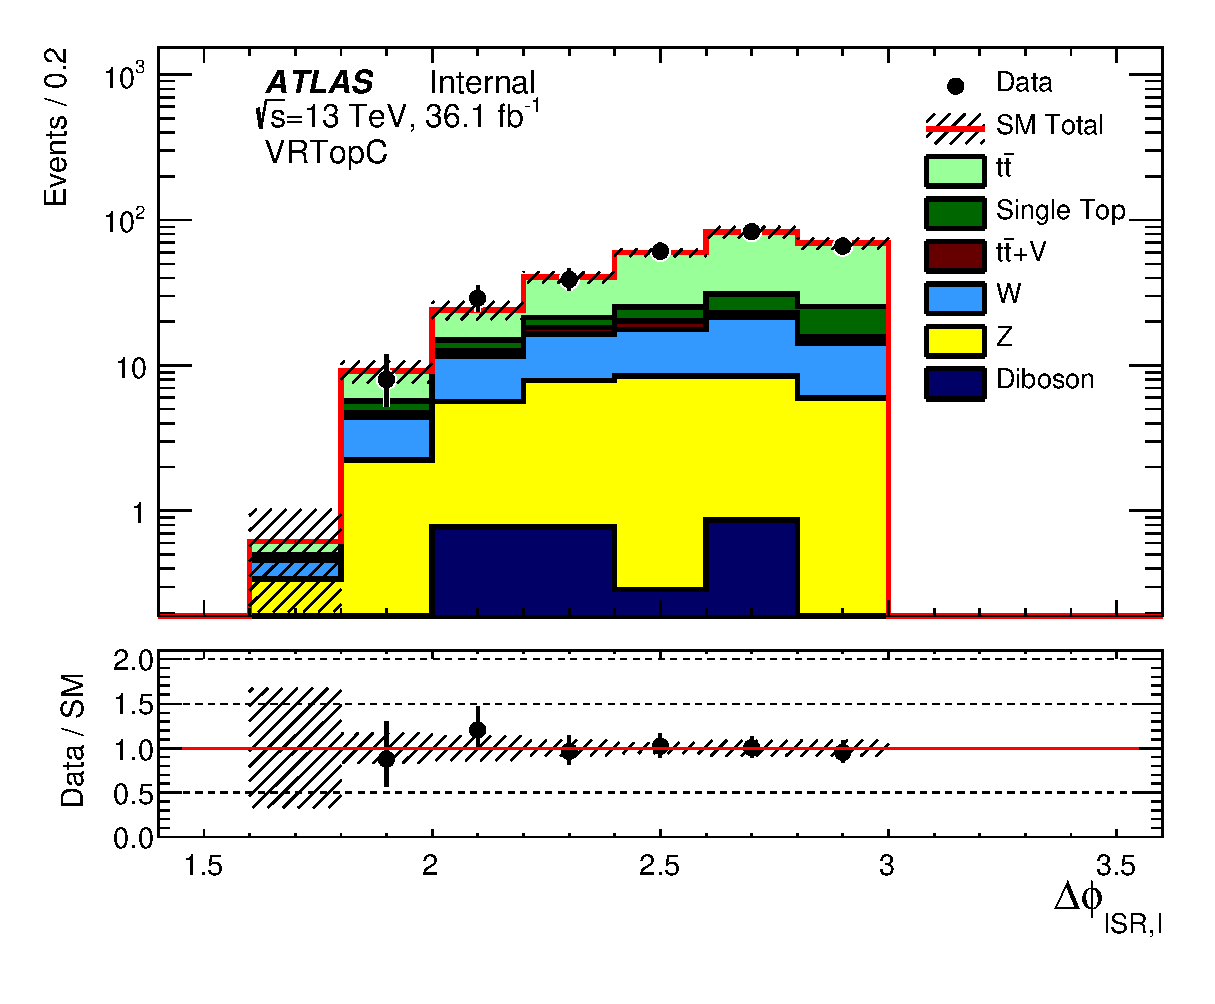
\includegraphics[width=0.45\textwidth]{figures/ttbar/postfit/CA_dphiISRI_VRTopC_log}
  \caption{\label{fig:ttbar0Lep1bVRISR}{Distribution of ISR signal region
      sensitive variables selections in the zero-lepton \ttbar\ validation
      region.}}
\end{figure}

\indent The agreement between data and MC prediction in the VR after applying the CR scale factor is better then 1 sigma.  The $\RISR$  shape seems to be well modeled as we see no distinct trends in the data vs MC ratio in $\RISR$. \\
\indent This agreement both in magnitude and shape demonstrates two things.  One, the ttbar control region indeed does correctly measure the amount of ttbar plus strong ISR that exists in both signal and validation region.  Two, the sub-dominant background predictions also cannot by wrong by more than around 100 percent.  For example we clearly would see disagreement in between data vs MC in this VR if the MC underestimated W+jets or Z+jets background by 100 percent.  Both of these facts gives us confidence that the predictions for the amount of background in the signal region is correct. \\